\FloatBarrier

\subsection{Investigation of field regions}

\todo[inline]{Update field plots}

In this section, the influence of the field region described in \autoref{sec:rad_fields} on the dipole moments are investigated. Making the TEM cell larger, such that $k\cdot r > 1$, is hardly possible without enabling higher-order modes to propagate. On the other hand, making the TEM cell smaller such that $k\cdot r \ll 1$, proves to be feasible. The following simulations are conducted with a TEM cell of dimensions $a=10\,\mathrm{mm}$ and $b=6\,\mathrm{mm}$, visible in \autoref{fig:krtemcell}.  

\begin{figure}[h]
	\centering
	\includegraphics[width=0.7\linewidth]{content/img/kr_tem_cell}
	\caption{TEM cell containing dipole moments}
	\label{fig:krtemcell}
\end{figure}


First, the current loop antenna used in \autoref{sec:loop_sim} is placed in the dead center of the TEM cell. The equivalent dipole moments are shown in \autoref{fig:loop_small_tem_moments}. In the \autoref{fig:dipole_moments_loop_antenna_copy} next to it, the dipole moments of the same antenna in the larger TEM cell used before ($a=40\,\mathrm{mm}$ and $b=24\,\mathrm{mm}$) are presented. 

\todo{The e field approx. in the python code is based on the large TEM cell. Therefore, the magnitude of the dipole moments of the small TEM cell are probably off}
\begin{figure}[htbp]
	\centering
	\begin{minipage}[t]{0.48\textwidth}
	\centering
\includegraphics[width=1\linewidth]{content/img/loop_small_tem_moments.png}
\caption{Moments in small TEM cell}
\label{fig:loop_small_tem_moments}
	\end{minipage}
	\hfill
	\begin{minipage}[t]{0.48\textwidth}
	\centering
	\includegraphics[width=1\linewidth]{content/img/dipole_moments_loop_antenna.png}
	\caption{Moments in normal TEM cell}
	\label{fig:dipole_moments_loop_antenna_copy}
	\end{minipage}
\end{figure}

This is done to compare the dipole moments in both cases. While they clearly increased by magnitude in case of the small TEM cell due to better coupling, their non-linear frequency relation still remains. This means that the change of field regions is not the reason for this behavior.

\todo{Insert kr, describe where r is measured, describe why the suspicion was that kr could influence this and how the fields change in the regions as described in the theoretical parts. Insert small current loop simulation. Insert Dipole Moment Simulations}

The $k\cdot r$ factor is determined in \autoref{fig:kranalysissmalltem} in the frequency range from 1\,MHz to 3\,GHz for the small TEM cell. This factor does not surpass 0.1, thus fulfilling the requirement $k\cdot r \ll 1$ for this investigation. For comparison, the $k\cdot r$ factor over a wider frequency range are shown in \autoref{fig:kranalysissmalltem} for the normal sized TEM cell ($a = 40\,\mathrm{mm}$ and $b = 24\,\mathrm{mm}$) and a degenerately high TEM cell ($a = 10\,\mathrm{mm}$ and $b=44\,\mathrm{mm}$). The high TEM does not have a port impedance of $50\,\Omega$, and is an attempt to achieve a large $k\cdot r$ factor without higher-order modes propagating. The markers in \autoref{fig:kranalysis} indicate the cut-off frequency, in which the next higher-order mode propagates. They demonstrate, that even in the high TEM cell a $k\cdot r = 1$ is not achieved.


\begin{figure}[htbp]
	\centering
	\begin{minipage}[t]{0.48\textwidth}
	\centering
	\includegraphics[width=1\linewidth]{content/img/kr_analysis_small_TEM}
	\caption{$k\cdot r$ in small TEM cell}
	\label{fig:kranalysissmalltem}
	\end{minipage}
	\hfill
	\begin{minipage}[t]{0.48\textwidth}
	\centering
	\includegraphics[width=1\linewidth]{content/img/kr_analysis}
	\caption{$k\cdot r$ for other TEM cells}
	\label{fig:kranalysis}
	\end{minipage}
\end{figure}
\todo{Fix figures: Titles and Legends}

Now, three simulations are conducted with different excitation sources in the small TEM cell:

\begin{itemize}
	\item The current loop 
	\item The equivalent dipole sources $e_z$ and $m_m$ of the current loop
	\item The equivalent magnetic dipole source $m_m$, neglecting $e_z$
\end{itemize}

\autoref{fig:outputpowercomparisonsmalltem} shows the output power over frequency normalized to 1\,W for all three constellations. The normalization is done to qualitatively discuss the frequency-dependent coupling behavior. \autoref{fig:phaseshiftcomparisonsmalltem} demonstrates the phase shift between the powers at the two waveports over frequency.

\begin{figure}[htbp]
	\centering
	\begin{minipage}[t]{0.48\textwidth}
		\centering
		\includegraphics[width=1\linewidth]{content/img/output_power_comparison_small_tem}
		\caption{Output powers}
		\label{fig:outputpowercomparisonsmalltem}
	\end{minipage}
	\hfill
	\begin{minipage}[t]{0.48\textwidth}
		\centering
		\includegraphics[width=1\linewidth]{content/img/phase_shift_comparison_small_tem}
		\caption{Phase shifts}
		\label{fig:phaseshiftcomparisonsmalltem}
	\end{minipage}
\end{figure}

The frequency dependent behavior of the output power does not change depending on the type of dipole moment used. This is significant, because this shows that the dipole moments do not exhibit different coupling behaviors in the TEM cells. This is further proven in the phase shift plots. The magnetic dipole moment causes a constant phase shift of $-\pi$. If this was not the case, this would mean that the coupling behavior of the magnetic dipole moment in the TEM cell would change. Since the opposite is the case, this poses as good evidence against arguments of change in field regions causing the non-linear dipole moment behavior. Instead, it is very likely to be caused by the geometry of the antenna.


